\documentclass[11pt]{standalone}
\usepackage{tikz}
\usetikzlibrary{shapes.geometric}
\usetikzlibrary{plotmarks}
\usetikzlibrary{arrows.meta}
\begin{document} 

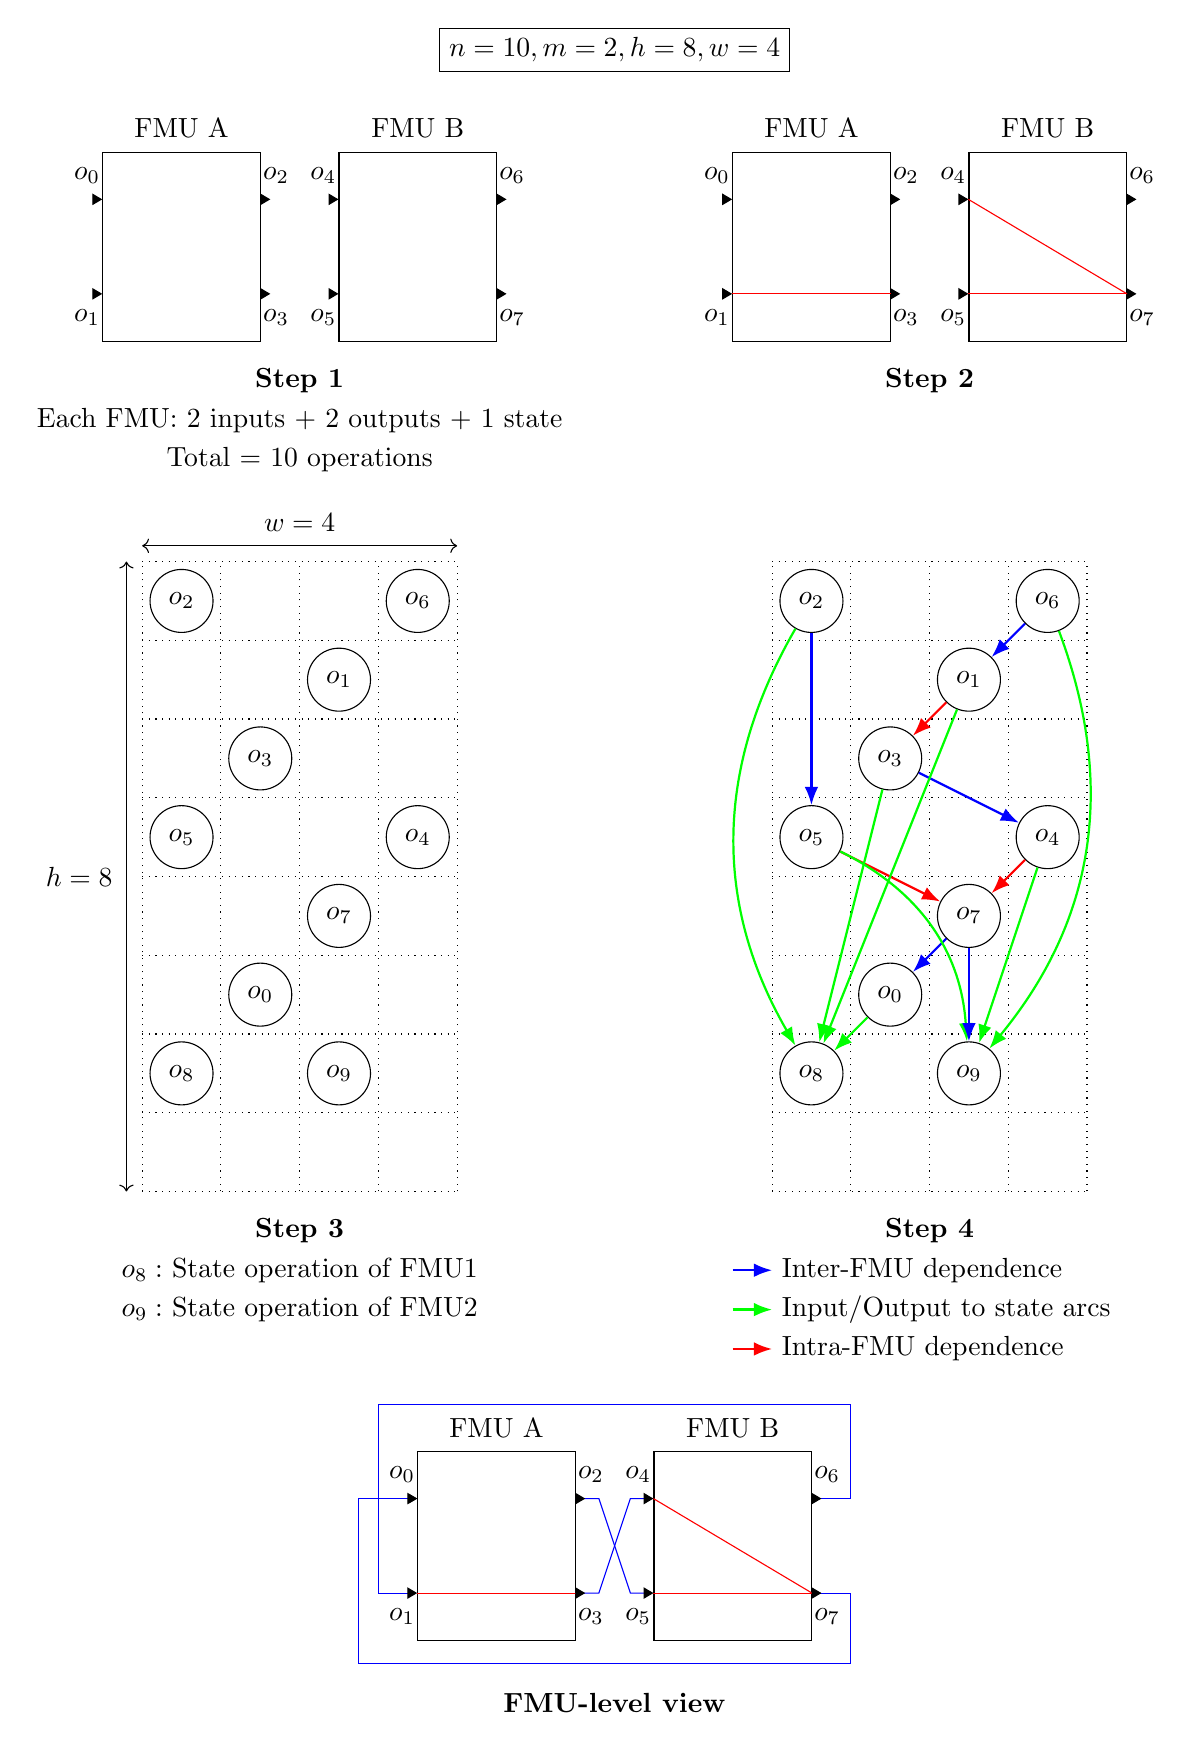
\begin{tikzpicture}
\begin{scope}
% FMU1
\node[rectangle,draw,minimum height = 2.4cm,minimum width = 2cm] (fmu1) {};
\draw[-{Triangle[]},shorten >=-2pt] ([yshift=0.6cm]fmu1.east) -- ([yshift=0.6cm,xshift=0.05cm]fmu1.east);
\draw[-{Triangle[]},shorten >=-2pt] ([yshift=-0.6cm]fmu1.east) -- ([yshift=-0.6cm,xshift=0.05cm]fmu1.east);
\draw[draw=white,-{Triangle[black]}] ([yshift=0.6cm,xshift=-0.1cm]fmu1.west) -- ([yshift=0.6cm]fmu1.west);
\draw[draw=white,-{Triangle[black]}] ([yshift=-0.6cm,xshift=-0.1cm]fmu1.west) -- ([yshift=-0.6cm]fmu1.west);
\node[below of=fmu1,yshift=2.5cm] {FMU A};
\node[left of=fmu1,yshift=0.9cm,xshift=-0.2cm] {$o_0$};
\node[left of=fmu1,yshift=-0.9cm,xshift=-0.2cm] {$o_1$};
\node[right of=fmu1,yshift=0.9cm,xshift=0.2cm] {$o_2$};
\node[right of=fmu1,yshift=-0.9cm,xshift=0.2cm] {$o_3$};
% FMU2
\node[rectangle,draw,minimum height = 2.4cm,minimum width = 2cm, xshift=3cm] (fmu2) {};
\draw[-{Triangle[]},shorten >=-2pt] ([yshift=0.6cm]fmu2.east) -- ([yshift=0.6cm,xshift=0.05cm]fmu2.east);
\draw[-{Triangle[]},shorten >=-2pt] ([yshift=-0.6cm]fmu2.east) -- ([yshift=-0.6cm,xshift=0.05cm]fmu2.east);
\draw[draw=white,-{Triangle[black]}] ([yshift=0.6cm,xshift=-0.2cm]fmu2.west) -- ([yshift=0.6cm]fmu2.west);
\draw[draw=white,-{Triangle[black]}] ([yshift=-0.6cm,xshift=-0.2cm]fmu2.west) -- ([yshift=-0.6cm]fmu2.west);
\node[below of=fmu2,yshift=2.5cm] {FMU B};
\node[left of=fmu2,yshift=0.9cm,xshift=-0.2cm] {$o_4$};
\node[left of=fmu2,yshift=-0.9cm,xshift=-0.2cm] {$o_5$};
\node[right of=fmu2,yshift=0.9cm,xshift=0.2cm] {$o_6$};
\node[right of=fmu2,yshift=-0.9cm,xshift=0.2cm] {$o_7$};

\node [yshift=-.5cm,xshift=1.5cm] at (fmu1.south) {\textbf{Step 1}};
\node [yshift=-1cm,xshift=1.5cm] at (fmu1.south) {Each FMU: 2 inputs + 2 outputs + 1 state};
\node [yshift=-1.5cm,xshift=1.5cm] at (fmu1.south) {Total = 10 operations};

\end{scope}

\begin{scope}[xshift=8cm]
% FMU1
\node[rectangle,draw,minimum height = 2.4cm,minimum width = 2cm] (fmu1) {};
\draw[-{Triangle[]},shorten >=-2pt] ([yshift=0.6cm]fmu1.east) -- ([yshift=0.6cm,xshift=0.05cm]fmu1.east);
\draw[-{Triangle[]},shorten >=-2pt] ([yshift=-0.6cm]fmu1.east) -- ([yshift=-0.6cm,xshift=0.05cm]fmu1.east);
\draw[draw=white,-{Triangle[black]}] ([yshift=0.6cm,xshift=-0.2cm]fmu1.west) -- ([yshift=0.6cm]fmu1.west);
\draw[draw=white,-{Triangle[black]}] ([yshift=-0.6cm,xshift=-0.2cm]fmu1.west) -- ([yshift=-0.6cm]fmu1.west);
\node[below of=fmu1,yshift=2.5cm] {FMU A};
\node[left of=fmu1,yshift=0.9cm,xshift=-0.2cm] {$o_0$};
\node[left of=fmu1,yshift=-0.9cm,xshift=-0.2cm] {$o_1$};
\node[right of=fmu1,yshift=0.9cm,xshift=0.2cm] {$o_2$};
\node[right of=fmu1,yshift=-0.9cm,xshift=0.2cm] {$o_3$};
\draw [draw=red]([yshift=-0.6cm]fmu1.west) -- ([yshift=-0.6cm]fmu1.east);
% FMU2
\node[rectangle,draw,minimum height = 2.4cm,minimum width = 2cm, xshift=3cm] (fmu2) {};
\draw[-{Triangle[]},shorten >=-2pt] ([yshift=0.6cm]fmu2.east) -- ([yshift=0.6cm,xshift=0.05cm]fmu2.east);
\draw[-{Triangle[]},shorten >=-2pt] ([yshift=-0.6cm]fmu2.east) -- ([yshift=-0.6cm,xshift=0.05cm]fmu2.east);
\draw[draw=white,-{Triangle[black]}] ([yshift=0.6cm,xshift=-0.2cm]fmu2.west) -- ([yshift=0.6cm]fmu2.west);
\draw[draw=white,-{Triangle[black]}] ([yshift=-0.6cm,xshift=-0.2cm]fmu2.west) -- ([yshift=-0.6cm]fmu2.west);
\node[below of=fmu2,yshift=2.5cm] {FMU B};
\node[left of=fmu2,yshift=0.9cm,xshift=-0.2cm] {$o_4$};
\node[left of=fmu2,yshift=-0.9cm,xshift=-0.2cm] {$o_5$};
\node[right of=fmu2,yshift=0.9cm,xshift=0.2cm] {$o_6$};
\node[right of=fmu2,yshift=-0.9cm,xshift=0.2cm] {$o_7$};
\draw [draw=red]([yshift=0.6cm]fmu2.west) -- ([yshift=-0.6cm]fmu2.east);
\draw [draw=red]([yshift=-0.6cm]fmu2.west) -- ([yshift=-0.6cm]fmu2.east);

\node [yshift=-.5cm,xshift=1.5cm] at (fmu1.south) {\textbf{Step 2}};

\end{scope}

\begin{scope}[yshift=-8cm,xshift=1.5cm]

\draw[step=1cm,dotted] (-2,-4) grid (2,4);
%level 1
\node[circle,draw,minimum size=.8cm] at(-1.5,3.5) {$o_2$};
\node[circle,draw,minimum size=.8cm] at(1.5,3.5) {$o_6$};
%level 3
\node[circle,draw,minimum size=.8cm] at(-.5,1.5) {$o_3$};
%level 5
\node[circle,draw,minimum size=.8cm] at(.5,-.5) {$o_7$};
%level 2
\node[circle,draw,minimum size=.8cm] at(-1.5,.5) {$o_5$};
\node[circle,draw,minimum size=.8cm] at(0.5,2.5) {$o_1$};
%level 4
\node[circle,draw,minimum size=.8cm] at(1.5,.5) {$o_4$};
%level 6
\node[circle,draw,minimum size=.8cm] at(-.5,-1.5) {$o_0$};
%level 7
\node[circle,draw,minimum size=.8cm] at(.5,-2.5) {$o_9$};
\node[circle,draw,minimum size=.8cm] at(-1.5,-2.5) {$o_8$};

\draw[<->] (-2.2,-4) -- node [xshift=-0.6cm]{$h = 8$} (-2.2,4);
\draw[<->] (-2,4.2) -- node [yshift=0.3cm]{$w = 4$} (2,4.2);

\node at(0,-4.5) {\textbf{Step 3}};
\node at(0,-5) {$o_8:$ State operation of FMU1};
\node at(0,-5.5) {$o_9:$ State operation of FMU2};

\end{scope}

\begin{scope}[yshift=-8cm,xshift=9.5cm]

\draw[step=1cm,dotted] (-2,-4) grid (2,4);
%level 1
\node[circle,draw,minimum size=.8cm] at(-1.5,3.5) (o2) {$o_2$};
\node[circle,draw,minimum size=.8cm] at(1.5,3.5) (o6) {$o_6$};
%level 3
\node[circle,draw,minimum size=.8cm] at(-.5,1.5) (o3) {$o_3$};
%level 5
\node[circle,draw,minimum size=.8cm] at(.5,-.5) (o7) {$o_7$};
%level 2
\node[circle,draw,minimum size=.8cm] at(-1.5,.5) (o5) {$o_5$};
\node[circle,draw,minimum size=.8cm] at(0.5,2.5) (o1) {$o_1$};
%level 4
\node[circle,draw,minimum size=.8cm] at(1.5,.5) (o4) {$o_4$};
%level 6
\node[circle,draw,minimum size=.8cm] at(-.5,-1.5) (o0) {$o_0$};
%level 7
\node[circle,draw,minimum size=.8cm] at(.5,-2.5) (o9) {$o_9$};
\node[circle,draw,minimum size=.8cm] at(-1.5,-2.5) (o8) {$o_8$};

%Inter-FMU
\draw [-{Latex[]},draw=blue,line width=.8pt] (o2) -- (o5);
\draw [-{Latex[]},draw=blue,line width=.8pt] (o3) -- (o4);
\draw [-{Latex[]},draw=blue,line width=.8pt] (o7) -- (o0);
\draw [-{Latex[]},draw=blue,line width=.8pt] (o6) -- (o1);

%Intra-FMU
\draw [-{Latex[]},draw=red,line width=.8pt] (o1) -- (o3);
\draw [-{Latex[]},draw=red,line width=.8pt] (o4) -- (o7);
\draw [-{Latex[]},draw=red,line width=.8pt] (o5) -- (o7);

%To state
\path (o2) edge[-{Latex[]},bend right,draw=green,line width=.8pt] (o8);
\path (o3) edge[-{Latex[]},draw=green,line width=.8pt] (o8);
\path (o0) edge[-{Latex[]},draw=green,line width=.8pt] (o8);
\path (o1) edge[-{Latex[]},draw=green,line width=.8pt] (o8);

\path (o4) edge[-{Latex[]},draw=green,line width=.8pt] (o9);
\path (o5) edge[-{Latex[]},bend left,draw=green,line width=.8pt] (o9);
\path (o6) edge[-{Latex[]},bend left,draw=green,line width=.8pt] (o9);
\path (o7) edge[-{Latex[]},draw=blue,line width=.8pt] (o9);

\node [anchor=west,xshift=-2cm] at(0,-5) (exp1) {Inter-FMU dependence};
\draw [-{Latex[]},draw=blue,line width=.8pt] ([xshift=-.5cm]exp1.west) -- (exp1);

\node [anchor=west,xshift=-2cm] at(0,-5.5) (exp2) {Input/Output to state arcs};
\draw [-{Latex[]},draw=green,line width=.8pt] ([xshift=-.5cm]exp2.west) -- (exp2);

\node [anchor=west,xshift=-2cm] at(0,-6) (exp3) {Intra-FMU dependence};
\draw [-{Latex[]},draw=red,line width=.8pt] ([xshift=-.5cm]exp3.west) -- (exp3);

\node at(0,-4.5) {\textbf{Step 4}};
\end{scope}

\begin{scope}[yshift=-16.5cm,xshift=4cm]
% FMU1
\node[rectangle,draw,minimum height = 2.4cm,minimum width = 2cm] (fmu1) {};

\draw[draw=white,-{Straight Barb[angle=60:2pt 3,black]}] ([yshift=0.6cm,xshift=-0.2cm]fmu1.west) -- ([yshift=0.6cm]fmu1.west);
%\draw[draw=white,-{Straight Barb[angle=60:2pt 3,black]}] ([yshift=-0.6cm,xshift=-0.2cm]fmu1.west) -- ([yshift=-0.6cm]fmu1.west);
\node[below of=fmu1,yshift=2.5cm] {FMU A};
\node[left of=fmu1,yshift=0.9cm,xshift=-0.2cm] {$o_0$};
\node[left of=fmu1,yshift=-0.9cm,xshift=-0.2cm] {$o_1$};
\node[right of=fmu1,yshift=0.9cm,xshift=0.2cm] {$o_2$};
\node[right of=fmu1,yshift=-0.9cm,xshift=0.2cm] {$o_3$};
\draw [draw=red]([yshift=-0.6cm]fmu1.west) -- ([yshift=-0.6cm]fmu1.east);
% FMU2
\node[rectangle,draw,minimum height = 2.4cm,minimum width = 2cm, xshift=3cm] (fmu2) {};

\node[below of=fmu2,yshift=2.5cm] {FMU B};
\node[left of=fmu2,yshift=0.9cm,xshift=-0.2cm] {$o_4$};
\node[left of=fmu2,yshift=-0.9cm,xshift=-0.2cm] {$o_5$};
\node[right of=fmu2,yshift=0.9cm,xshift=0.2cm] {$o_6$};
\node[right of=fmu2,yshift=-0.9cm,xshift=0.2cm] {$o_7$};
\draw [draw=red]([yshift=0.6cm]fmu2.west) -- ([yshift=-0.6cm]fmu2.east);
\draw [draw=red]([yshift=-0.6cm]fmu2.west) -- ([yshift=-0.6cm]fmu2.east);

%Inter-FMU
\coordinate [right of =fmu2, yshift=1.8cm,xshift=.5cm] (c1);
\coordinate [left of =fmu1, yshift=1.8cm,xshift=-.5cm] (c2);

\coordinate [right of =fmu2, yshift=-1.5cm,xshift=.5cm] (c3);
\coordinate [left of =fmu1, yshift=-1.5cm,xshift=-.75cm] (c4);

\draw [draw=blue,-{Triangle[black]}]([yshift=0.6cm]fmu2.east) -| (c1) -- (c2) |- ([yshift=-.6cm]fmu1.west);
\draw [draw=blue,-{Triangle[black]}]([yshift=-.6cm]fmu2.east) -| (c3) -- (c4) |- ([yshift=.6cm]fmu1.west);

\coordinate [right of =fmu1, yshift=-.6cm,xshift=.3cm] (c5);
\coordinate [left of =fmu2, yshift=.6cm,xshift=-.3cm] (c6);

\coordinate [right of =fmu1, yshift=.6cm,xshift=.3cm] (c7);
\coordinate [left of =fmu2, yshift=-.6cm,xshift=-.3cm] (c8);

\draw [draw=blue,-{Triangle[black]}]([yshift=-.6cm]fmu1.east) -- (c5) -- (c6) -- ([yshift=.6cm]fmu2.west);
\draw [draw=blue,-{Triangle[black]}]([yshift=.6cm]fmu1.east) -- (c7) -- (c8) -- ([yshift=-.6cm]fmu2.west);

\draw[-{Triangle[black]},shorten >=-2pt] ([yshift=0.6cm]fmu1.east) -- ([yshift=0.6cm,xshift=0.05cm]fmu1.east);
\draw[-{Triangle[black]},shorten >=-2pt] ([yshift=-0.6cm]fmu1.east) -- ([yshift=-0.6cm,xshift=0.05cm]fmu1.east);

\draw[-{Triangle[]},shorten >=-2pt] ([yshift=0.6cm]fmu2.east) -- ([yshift=0.6cm,xshift=0.05cm]fmu2.east);
\draw[-{Triangle[]},shorten >=-2pt] ([yshift=-0.6cm]fmu2.east) -- ([yshift=-0.6cm,xshift=0.05cm]fmu2.east);

\node[below of = fmu1,yshift=-1cm,xshift=1.5cm] {\textbf{FMU-level view}};
\end{scope}

\begin{scope}[yshift=2.5cm,xshift=5.5cm]
\node [draw] at(0,0) {$n = 10, m = 2, h = 8, w = 4$};
\end{scope}
\end{tikzpicture}

\end{document}